\section{Isomorphism}

When we compare two posets $\P$ and $\Q$ we might come to the conclusion that
they \emph{behave the same way}, that they \emph{have the same structure},
meaning that to go from poset $\P$ to poset $\Q$ only a bijection-like renaming
operation on the relation and the elements would have to be performed. In such
a case, we say that $\P$ and $\Q$ are \concept{isomorphic}.

Let us try to build an example. We want two posets $\P = (\S, \le_{\S})$ and $\Q =
(\T, \le_{\T})$ such that they are intrinsically different (because the case where
$\P = \Q$ is trivial) while their structures look the same. If we want two posets
to be different, at least one of $\S \neq \T$ or $\le_{\S} \neq \le_{\T}$ must be true.

For example, if we take the notations used in \sref{ex:poset:def:a} and we
define $\P$ a poset on the set $\enum{1, 2}$ and $\Q$ a poset on the set $\enum{1, 2, 3}$
we would not be able to find a bijection between the two posets $\P$ and $\Q$
because the cardinality of their respective sets differ.

\begin{table}
\centering
\caption{Mapping $\phi$ of $\P$ to $\Q$.}
\label{table:poset:iso:a}
\begin{tabular}{c|c}
	$x$ & $\phi(x)$ \\
	\hline
	1 & 1 \\
	2 & 2 \\
	3 & 4 \\
\end{tabular}
\end{table}

\begin{table}
\centering
\caption{Applying mapping $\phi$ shows that the structure of the two posets is
the same.}
\label{table:poset:iso:b}
\begin{tabular}{c|c}
	$\P$ & $\Q$\\
	\hline
	$1 \le 1$   & $1 \le 1$\\
	$1 \le 2$   & $1 \le 2$\\
	$1 \le 3$   & $1 \le 4$\\
	$2 \nleq 1$ & $2 \nleq 1$\\
	$2 \le 2$   & $2 \le 2$\\
	$2 \le 3$   & $2 \le 4$\\
	$3 \nleq 1$ & $4 \nleq 1$\\
	$3 \nleq 2$ & $4 \nleq 2$\\
	$3 \le 3$   & $4 \le 4$\\
\end{tabular}
\end{table}

Since we need sets of the same cardinality, let us define the sets $\S = \enum{1, 2,
3}$ (the set of $\P$) and $\T = \enum{1, 2, 4}$ (the set of $\Q$). If we consider
the relation $\le_{\S} = \le_{\T} = \le$ we can construct a table mapping elements of
$\P$ to elements of $\Q$, we name this mapping $\phi$, in such a way that $x
\le_{\S} y \iff \phi(x) \le_{\T} \phi(y)$. \Cref{table:poset:iso:a,table:poset:iso:b}
prove that the construction of this mapping is possible.

\begin{figure}
	\centering
	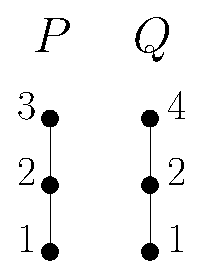
\includegraphics[width=0.2\textwidth]{fig/poset/iso/a}
	\caption{Illustration of two isomorphic posets.}
	\label{fig:poset:iso:a}
\end{figure}

\ref{fig:poset:iso:a} shows two small
diagrams\footnote{The diagrams of \ref{fig:poset:iso:a} are Hasse diagrams. In those diagrams, we
notice that edges that can be deduced by the transitivity property are not
drawn. The topic of Hasse diagrams is covered in detail in
\Cref{tree:poset:hasse}.}
for the example we just gave.
Those diagrams provide an illustration of what we mean by \emph{posets having
the same structure}. Looking at a poset ($\P$ or $\Q$), an edge from an upper
node $x$ to a lower node $y$ implies that $x R y$ holds, where $R$ is the order
of the considered poset.

We currently only gave examples of finite posets. We could show what can be
achieved with infinite posets. For this example we choose $\S = \T = \R$,
$\le_{\S} = \le$ and $\le_{\T} = \ge$. We notice that by negating the relation
$\le_{\S}$ and thus mapping $x \in \R$ in $\S$ to $-x$ in $\T$ we get a
bijection between the sets of $\S$-relations and $\T$-relations, namely for all
$x, y \in \R$ we have $x \le y \iff -x \ge -y$.

In general, posets must have the \emph{same size} to be isomorphic. This remark
is trivial for finite sets, but for infinite sets, countable sets cannot be
isomorphic to uncountable sets and vice versa. Another general remark is that
those posets must have the same bounds, e.g. a closed interval cannot be
isomorphic to an open interval and vice versa because a closed interval has a
least and greatest element, while an open one has not (see
\Cref{tree:poset:leastandgreatest} for an illustration).

We now understand what isomorphism means for posets and can give a formal
definition.
\begin{definition}[Isomorphic posets]
Two posets $\P$ and $\Q$ are isomorphic\define{isomorphic}, denoted $\P \cong \Q$, if
there exists an \emph{order-preserving bijection} $\phi : \P \to \Q$ whose
inverse is order-preserving; that is, $$s \leq t~\text{in}~\P \iff \phi(s) \leq
\phi(t)~\text{in}~\Q.$$ For example, if $B_{\S}$ denotes the poset of all subsets
of the set $\S$ ordered by inclusion, then $B_{\S} \cong B_{\T}$ whenever $\card{\S} =
\card{\T}$.
\end{definition}
